\section{\thesection.~Computational Music Analysis}

\note[itemize]{
  \item Before I will present some of the core aspects of my research, I would like to
  explain what I understand under Computational Music Analysis.
}

\begin{frame}<1-2>[label=cma]{\insertsectionhead}

  Potential of Computational Music Analysis
  \begin{enumerate}
    \item<2-> complementing music theory (e.g., addressing potential biases)
    \note<2->{sampling bias in contemporary and present-day sources}
    \item<3-> resolving ambiguities in terminology
    \item<4-> empirically validating theoretical assumptions \& asking entirely new questions
  \end{enumerate}


  % \begin{itemize}
  %   \item<1-> Computational Music Analysis \textcolor{epflred}{$\neq$} Music Analysis with a Computer
  %   \item<2-> Many ``music theories'' for various aspects of music (harmony, meter, form, \ldots)
  %   \item<3-> Interaction and integration is difficult
  %   \item<4-> Using a computer can be useful
  %     \begin{itemize}
  %       \item<4-> analysing more pieces faster
  %       \item<4-> forcing formalization $\rightarrow$ consistency in analytical decisions
  %     \end{itemize}
  %   \item<5-> Empirical testing
  %     \begin{itemize}
  %       \item<5->Music Perception and Cognition \citep[e.g.][]{Huron2016}
  %       \item<5->Corpus Studies \citep[e.g.][]{Shanahan2020}
  %     \end{itemize}

    % \item Problem: No interfaces! (few counterexamples: NRT \& Form \citep{Horton2018})
    % \item Ideally, it would be specified how all of them interact,
    % advancing Music Theory to a Theory of Music

    % \item<2-> Empirically testing music theory \citep{Temperley2001,Huron2016,Moss2019a}
    % \item<2-> psychological constraints do not solely account for all aesthetic decisions, e.g. Tallis example \citep{Moss2017}
    % \item<2-> Corpus Studies \citep{Shanahan2020} $\rightarrow$ Models!
    %   \begin{itemize}
    %     \item models for musical sequences: Syntax \citep{Bernstein1976,Lerdahl1983,Rohrmeier2011}
    %     \item models for relations between musical notes, Tonal Spaces \citep{Lerdahl2001,Tymoczko2011,Cohn2012} % Hauptmann, Riemann, v. Oettingen, Hostinský
    %   \end{itemize}
  % \end{itemize}
\end{frame}

% \note[itemize]{
%   \item{Maybe the most important thing to take away from my presentation is that}
%     Computational Music Analysis is not the same as Music Analysis with a computer.
%   \item In fact, many aspects of what I am going to present could be perfectly done without using a machine.
%   \item It is more a different way to approach Music Analysis
%   \item and crucially relies on describing all relevant elements and their relations with each other
%     in an explicit manner.
%   \item Such a description, often given in formal or mathematical terms, is a \emph{Computational Model} of some phenomenon.
%   \item A computational model does not need to be perfect or comprehensive. It can always be altered and improved,
%       but its main advantage to other, less formal approaches is that it prevents arbitrary \emph{ad hoc} decisions
%       that often prevail in Music Analysis.
%   \item That being said, using a computer in order to work with such a model can be incredibly useful.
%   \item Schenkerian Theory~\citep{Cadwallader1998}, Neo-Riemannian Theory~\citep{Cohn1998},
%     Tonal Pitch Space~\citep{Lerdahl2001}, Classical Form~\citep{Caplin1998}
% }

\begin{frame}{\insertsectionhead}
  \begin{figure}
    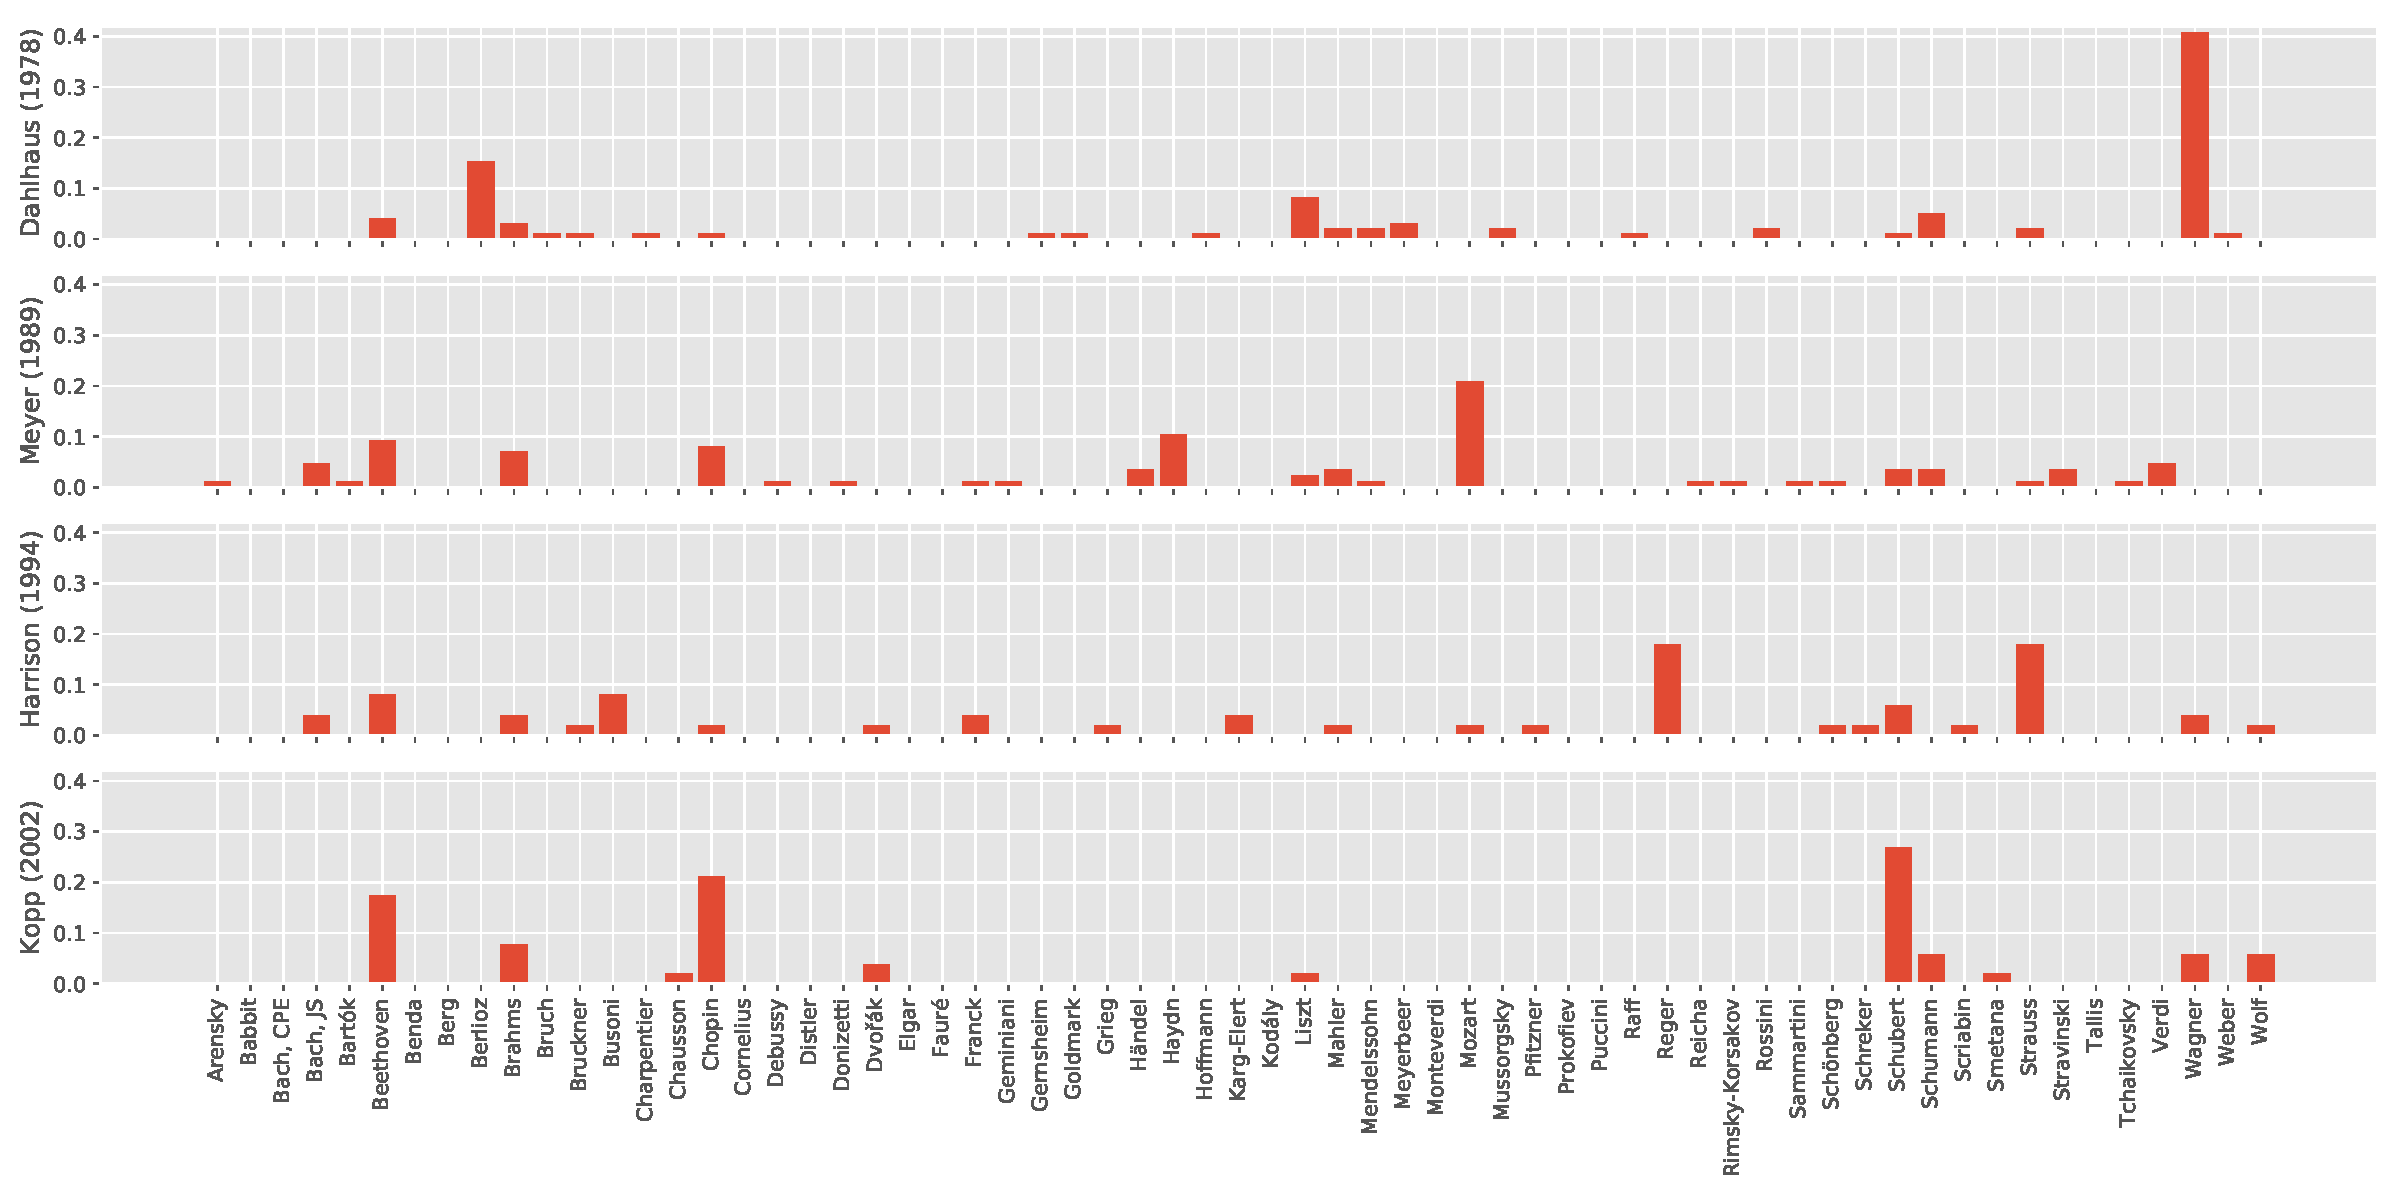
\includegraphics[width=.9\textwidth]{img/composer_counts.pdf}
    % \caption{}
    % \label{}
  \end{figure}
\end{frame}

\note[itemize]{
\item drawn conclusions may solely rely on different examples
\item implicit knowledge is inaccessible
}

\againframe<3>{cma}

\begin{frame}{\insertsectionhead}
  	\textbf{Definitions of Tonality}

   \begin{quote}
     ``the term is sometimes used as an equivalent for what Rousseau called
     a \emph{sistême musicale}, a rational and self-contained arrangement of musical phenomena''\\
     % [\ldots]. While tonality \emph{qua} system constitutes a theoretical
     % (and thus imaginative) abstraction from actual music, it is often hypostatized in
     % musicological discourse, converted from a theoretical structure into a musical reality.''\\
     \emph{\hfill\parencite{Hyer2001}}
  \end{quote}
  \vspace{1em}
  \pause
  \begin{quote}
    ``the relations between musical elements, e.g. notes or chords in a corpus''\\
    \emph{\hfill\parencite{Moss2019a}}
   \end{quote}
  % \onslide<2->{
  % \large
  % \begin{center}
  %   computational modeling $\color{epflred}{\Longleftrightarrow}$ corpus studies
  % \end{center}
  % }
\end{frame}

\note[itemize]{
  \item I like a definition by Brian Hyer in \emph{The New Grove Dictionary of Music and Musicians}.
}

\againframe<4->{cma}

% \begin{frame}<1-5>[label=disciplines]{\insertsectionhead}
%   \begin{center}
%     \begin{tikzpicture}
%       \node [visible on=<2->] (MT) at (0,0) {Music Theory};
%       \note[item]<2->{Music theory is the overarching framework}
%
%       \node [visible on=<3->] (part) at (-3,-4) {particular};
%       \draw[<->, >=stealth, line width=2, epfldark,visible on=<3->] (MT) -- (part) node [midway, sloped, above, epfldark] {Music Analysis};
%       \note[item]<3->{Music analysis looks at individual pieces, the particular}
%
%       \node [visible on=<4->] (gen) at (3, -4) {general};
%       \draw[<->, >=stealth, line width=2,  epfldark,visible on=<4->] (MT) -- (gen) node [midway, sloped, above, epfldark] {Corpus Studies};
%       \note[item]<4->{Corpus studies look at entire repertoires, aiming at describing the general.}
%
%       \draw[<->, >=stealth, line width=2, visible on=<5->] (part) -- (gen) node [visible on=<5->,align=center, midway,below] {Computational\\ Music Analysis}; % (CMA) at (0,-2.5)
%
%       \note[item]<5->{The mediating device are (formal) models. This is where my main research focus lies.}
%
%       \draw[<->, >=stealth, epflred, line width=2, visible on=<{6,8-}>] (MT) -- (gen);
%       \draw[<->, >=stealth, epflred, line width=2, visible on=<7->] (part) -- (gen);
%       \draw[<->, >=stealth, epflred, line width=2, visible on=<9>] (part) -- (MT);
%
%     \end{tikzpicture}
%   \end{center}
% \end{frame}
%
% \note[itemize]{
% \item Sampling bias can be addressed with Corpus Studies.
% \item Larger and common data
% \item instead of choosing suitable samples
% }
